\chapter{Graphen}

Ein Graph ist eine Struktur, die verwendet wird, um Beziehungen zwischen Objekten darzustellen.
Die Idee, Objekte durch Verbindungen zu verknüpfen, bildet die Grundlage für viele Anwendungen, unter anderem der Routenplanung.
\autoref{graphs:fig:beispielgraph} zeigt einen Graphen, welcher im folgenden für Beispiele benutzt wird.

\begin{figure}[ht]
    \centering
    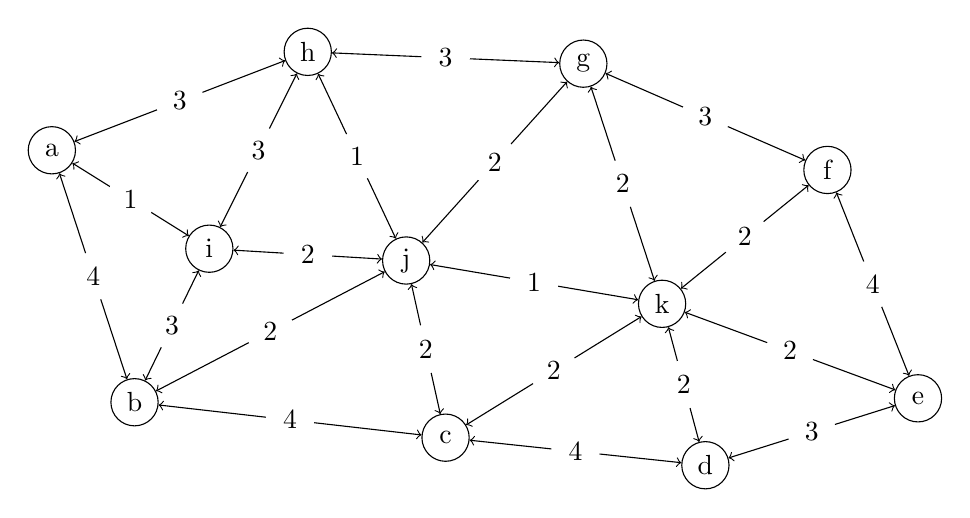
\begin{tikzpicture}
        % Nodes
        \node[circle, draw, minimum size=0.6cm, inner sep=0pt] at (0.5* 0.0, 0.5* 8.5)  (a)    {a};
        \node[circle, draw, minimum size=0.6cm, inner sep=0pt] at (0.5* 2.1, 0.5* 2.1)  (b)    {b};
        \node[circle, draw, minimum size=0.6cm, inner sep=0pt] at (0.5* 10.0, 0.5* 1.2)  (c)    {c};
        \node[circle, draw, minimum size=0.6cm, inner sep=0pt] at (0.5* 16.6, 0.5* 0.5)  (d)    {d};
        \node[circle, draw, minimum size=0.6cm, inner sep=0pt] at (0.5* 22.0, 0.5* 2.2)  (e)    {e};
        \node[circle, draw, minimum size=0.6cm, inner sep=0pt] at (0.5* 19.7, 0.5* 8.0)  (f)    {f};
        \node[circle, draw, minimum size=0.6cm, inner sep=0pt] at (0.5* 13.5, 0.5* 10.7)  (g)    {g};
        \node[circle, draw, minimum size=0.6cm, inner sep=0pt] at (0.5* 6.5, 0.5* 11.0)  (h)    {h};
        \node[circle, draw, minimum size=0.6cm, inner sep=0pt] at (0.5* 4.0, 0.5* 6.0)  (i)    {i};
        \node[circle, draw, minimum size=0.6cm, inner sep=0pt] at (0.5* 9.0, 0.5* 5.7)  (j)    {j};
        \node[circle, draw, minimum size=0.6cm, inner sep=0pt] at (0.5* 15.5, 0.5* 4.6)  (k)    {k};


        \draw[<->]  (a) edge node[circle, fill=white] {4} (b);
        \draw[<->]  (a) edge node[circle, fill=white] {3} (h);
        \draw[<->]  (a) edge node[circle, fill=white] {1} (i);

        \draw[<->]  (b) edge node[circle, fill=white] {4} (c);
        \draw[<->]  (b) edge node[circle, fill=white] {3} (i);
        \draw[<->]  (b) edge node[circle, fill=white] {2} (j);

        \draw[<->]  (c) edge node[circle, fill=white] {4} (d);
        \draw[<->]  (c) edge node[circle, fill=white] {2} (j);
        \draw[<->]  (c) edge node[circle, fill=white] {2} (k);

        \draw[<->]  (d) edge node[circle, fill=white] {3} (e);
        \draw[<->]  (d) edge node[circle, fill=white] {2} (k);

        \draw[<->]  (e) edge node[circle, fill=white] {4} (f);
        \draw[<->]  (e) edge node[circle, fill=white] {2} (k);

        \draw[<->]  (f) edge node[circle, fill=white] {3} (g);
        \draw[<->]  (f) edge node[circle, fill=white] {2} (k);

        \draw[<->]  (g) edge node[circle, fill=white] {3} (h);
        \draw[<->]  (g) edge node[circle, fill=white] {2} (j);
        \draw[<->]  (g) edge node[circle, fill=white] {2} (k);

        \draw[<->]  (h) edge node[circle, fill=white] {3} (i);
        \draw[<->]  (h) edge node[circle, fill=white] {1} (j);

        \draw[<->]  (i) edge node[circle, fill=white] {2} (j);

        \draw[<->]  (j) edge node[circle, fill=white] {1} (k);
    \end{tikzpicture}
    \caption{Beispielgraph}
    \label{graphs:fig:beispielgraph}
\end{figure}

\section{Definitionen}
Damit in den nachfolgenden Kapiteln sinnvoll argumentiert werden kann, ist es notwendig, einige Begriffe zu definieren.

\begin{definition}[Graph]
    Sofern nicht anders angegeben wird im folgenden Graph als eine Bezeichnung für einen endlichen, gerichteten Graph mit Kantengewichten, ohne Mehrfachkanten und Schleifen, verwendet.

    Als Schreibweise wird $G = (V, E)$ verwendet, wobei $V$ die Knotenmenge und $E$ die Kantenmenge ist. Eine Kante ist ein Tupel $(t, h, w)$. $t \in V$ wird als \emph{Fuß}, $h \in V$ als \emph{Kopf} und $w \in \mathbb{R}^+$ als \emph{Gewicht} bezeichnet. Gelegentlich wird auch nur $(t, h)$ geschrieben, um auszudrücken, dass zwei Knoten verbunden sind. Da ein Graph keine Mehrfachkanten zulässt, definiert diese Schreibweise auch eindeutig das Kantengewicht.

    Wird $G$ als ungerichtet bezeichnet, dann gilt $(t, h, w) \in E \Leftrightarrow (h, t, w) \in E$.
\end{definition}

\begin{definition}[Nachbar]
    Sei $G = (V, E)$. Ein Knoten $u \in V$ heißte \emph{Vorgänger} eines Knoten $v \in V$ wenn $(u, v) \in V$. $v$ ist in dann ein \emph{Nachfolger} von $u$. Ist $G$ ungerichtet spricht man beides mal von \emph{Nachbarn}.
\end{definition}

In einem Graphen gibt es oft das Interesse, von einem Knoten zu einem anderen zu gelangen.

\begin{definition}[Pfad]
    Ein Pfad auf einem Graph $G = (V, E)$ ist eine Folge von Knoten $v_1, \dotsc, v_n$, für die gilt, dass benachbarte Knoten im Pfad durch eine Kante in $G$ verbunden sind.
    Der Knoten $v_1$ wird Startknoten, $v_n$ Zielknoten genannt.
    Die Summe der Kantengewichte aller Kanten $(v_i, v_{i + 1})$ wird \emph{Länge} genannt.
    Die Anzahl Kantennutzungen $n - 1$ wird \emph{Hop-Länge} genannt.
\end{definition}

Zwischen zwei Knoten kann es Pfade unterschiedliche Länge geben.

\begin{definition}[Kürzester Pfad]
    Ein Pfad $v_1, \dotsc, v_n$ ist \emph{ein kürzester Pfad}, wenn die Länge des Pfades unter allen Pfad von $v_1$ nach $v_n$ minimal ist. Die Länge des kürzesten Pfades wird als \emph{Abstand} von $v_1$ und $v_n$ bezeichnet. Die Definition des Graphen lässt es zu, dass es mehrere kürzeste Pfade zwischen zwei Knoten gibt.

    Sei $P \subset V \times V$ die Menge der Knoten, zwischen denen ein Pfad existiert. Dann sind definiert:
    \begin{enumerate}
        \item
              ${spd} \colon P \to \mathbb{R}^+$ weist einem Knotenpaar den Abstand zu.

        \item
              ${sp} \colon P \to V \times V \times \dots \times V$ weist einem Knotenpaar einen kürzesten Pfad zu.
    \end{enumerate}
\end{definition}

\begin{definition}[Umkehrgraph]
    Sei $G = (V, E)$ ein Graph. Dann ist $G^T = (V, E^T)$ mit $(t, h, w) \in E \Leftrightarrow (h, t, w) \in E^T$ der \emph{Umkehrgraph} von $G$.
\end{definition}

Zusätzlich zum Finden eines Pfades zwischen zwei Knoten ist es häufig notwendig die kürzesten Pfade von einem Knoten zu allen anderen Knoten zu finden.
Auch die Umkehrung dieses Problem ist Interessent, also die kürzesten Pfade von allen Knoten zu einem Knoten zu bestimmen.
Diese Probleme sind äquivalent, da das Finden aller kürzesten Pfade zu einem Knoten auf einem Graph $G$ dem Finden aller kürzester Pfade auf dem Umkehrgraph $G^T$ entspricht.

\section{Graphenklassen}
\subsection{Straßengraphen}

Straßengraphen bilden eine besondere Klasse von Graphen und habe einige Eigenschaften, welche nicht alle Graphen haben.
Unter anderem
Sie sind nahezu planar (Über- und Unterführungen ausgenommen), haben einen kleinen Durschnittlichen Grad und eine hierarische Struktur:
Fahren von A nach B führt auf immer schneller Straßen bis zu einem gewissen Punkt, dann immer langsamere Straßen.
Insbesondere führt ab einer hinreichend großen Distanz der kürzeste Pfad zu einem großen Teil über die Autobahn.
Diese Eigenschaft lässt sich für das Wegfinden ausnutzen.

\subsection{Nicht-Straßen Graphen}

Formale Defintion Sichtbarkeitrgraphen.

Euklidische Ebene.
Polygone in der Ebene.

Gummiband Eigenschaft?

\subsubsection{Die Graphen im Detail}

\todo{Bilder}

\section{Dijkstra Algorithmus}

Als Baseline für das suchen verwende ich Dijkstra.
Später wird der Algorithmus auch benutzt werden.
Um die Kosten einer Suche nicht nur in Zeit auszudrücken wird noch definiert:
Die Mächtigkeit der Menge $u$ als Dijkstra Rank
Die Anzahl der Operationen \ref{graphs:dijkstra:pop} quqe pops.


\todo{Dijkstra Algorithmus erklären und Dijkstra Paper zitieren}

\begin{algorithm}[ht]
    \caption{Dijkstra Algorithmus}
    \begin{algorithmic}[1]
        \Require Graph $G = (V, E)$, Startknoten $s \in V$, Zielknoten $t \in V$
        \Ensure ${dist}$, ${pre}$
        \State // Initialisiere Distanz- und Vorgänger-Funktion
        \ForAll{$v \in V$}
        \State ${dist}(v) \leftarrow \infty$
        \State ${pre}(v) \leftarrow {none}$
        \EndFor


        \State
        \State // Initialisiere Vorrangwarteschlange
        \State ${dist}(s) \leftarrow 0$
        \State $Q\leftarrow \{ s \}$

        \State
        \While{$Q \neq \emptyset$}
        \State $u \leftarrow{extract\_min}(Q)$\label{graphs:dijkstra:pop}

        \State
        \State // Beende frühzeitig wenn Zielknoten gefunden wurde
        \If {$u = t$}
        \State \textbf{break}
        \EndIf

        \State
        \State // Aktualisiere Nachbarn
        \ForAll{$(u, v, w) \in E$}
        \If {${dist}(u) + w < {dist}(v)$}
        \State ${dist}(v) \leftarrow {dist}(u) + w$
        \State ${pre}(u) \leftarrow v$
        \State $Q = Q \cup \{ v \}$
        \EndIf
        \EndFor

        \EndWhile

        \State
        \State \Return ${dist}$, ${pre}$
    \end{algorithmic}
\end{algorithm}


\section{Dateiformat}

Die in dieser Arbeit verwendeten Graphen sind im \emph{.fmi} Dateiformat gespeichert, welches wie folgt definiert ist:

\begin{definition}[FMI Dateiformat]
    Eine Datei im .fmi Format besteht aus den folgenden Zeilen (in der angegebenen Reihenfolge):
    \begin{enumerate}
        \item
              Beliebig viele Kommentarzeilen, die mit einem \# beginnen.

        \item
              Eine leere Zeile.

        \item
              Eine Zeile, die die Anzahl der Knoten enthält.

        \item
              Eine Zeile, die die Anzahl der Kanten enthält.

        \item
              Knoten-Zeilen im Format: \texttt{KnotenId1 KnotenId2 Breitengrad Längengrad Höhe}

        \item
              Kanten-Zeilen im Format: \texttt{FußId1 KopfId2 Gewicht Typ Geschwindigkeit}

    \end{enumerate}
\end{definition}

Für die in dieser Arbeit verwendeten Graphen sind die Felder für Höhe, Typ und Geschwindigkeit nicht von Bedeutung, sie enthalten jeweils den Wert 0.

Die bereitgestellten Graphen mussten vor ihrer Nutzung gereinigt und an die Implementierung angepasst werden.
Sie enthielten isolierte Knoten, und die Kantengewichte der Sichtbarkeitsgraphen waren als Gleitkommazahlen gespeichert.
Für die Anpassung wurde ein Python-Skript benutzt, das folgende Aufgaben durchführt:

\begin{itemize}
    \item
          Transformation der Kantengewichte.

    \item
          Entfernung isolierter Knoten.

    \item
          Anpassung der Knoten-IDs, sodass die Knoten-IDs im Sichtbarkeitsgraphen den Bereich $0, \dotsc, n$ und im triangulierten Graphen den Bereich $0, \dotsc, n + m$ umfassen.
\end{itemize}

Während der Untersuchung der triangulierten Graphen wurde festgestellt, dass einige Kanten ein Gewicht von 0 aufwiesen.
Diese Kanten wurden unverändert beibehalten.

\todo{Plot degree before after}

\section{Datenstrukturen}

Vertices sind natürliche Zahlen bzw uint32.
Ein Graph enthält idealerweise keine isolierten Knoten.
isolierte Knoten sind doof für dijkstra und co.
Die Menge der Knoten ist definiert durch Ihre Anzahl.
Gibt es $n \in \mathbb{N}$ Knoten, so sind es $0, \dotsc, n - 1$.

Ein Graph der diese Eigenschaft nicht erfüllt, kann durch eine Mapping der Knoten in die Form gebracht werden
Hierfür wurde ein python script geschrieben
\todo{Vergleiche degree histogramme}

Jenachdem was mit dem Graph gemacht werden soll, sind verschiedene Eigenschaften von Vorteil.
Manchmal ist eine effiziente Nachbar Abfrage wichtig,
Manchmal das bearbeiten des Graphes, einfügen oder löschen von Knoten

Es wurde ein dyn Trait benutzt, welches eine Overhead hat und kein inlining zulässt.
Dafür lassen sich verschiedene Methoden vergleichen.

Die Grundlegenden Implementierungen kennen nur ihre Vorgänger.
Ein Reversibe Graph besteht aus einem Graph und seinem Umkehrgraph.
Gleiche Datenstruktur.

\subsection{VecVecGraph}
Mäßig schnelle Queries
Einfügen mit suche.
Bei vielen Knoten teuer.

\subsection{VecHashMap}
Besser Indexmap???

Eher langsame Queries.
Einfügen in O(1).

\subsection{VecGraph}
Schnelle Querries.
Einfügen sehr teuer.

